\documentclass{beamer}


\usepackage{amsmath}
\usepackage[style=alphabetic,url=true]{biblatex}
\usepackage{environ}
\usepackage{geometry}
\usepackage{graphicx}
\usepackage{tikz}
\usepackage[T2A]{fontenc}
\usepackage[utf8]{inputenc}
\usepackage[cache=false]{minted}
\usepackage{amsmath}
\usepackage{amsfonts}
\usepackage{amssymb}
\usepackage{calrsfs}
\usepackage{animate}
\usepackage{xmpmulti}


% \usetheme{Bergen}

\usecolortheme{beaver}

\setbeamertemplate{itemize item}[circle]
\setbeamertemplate{itemize subitem}{--}
\addtobeamertemplate{navigation symbols}{}{
  \usebeamerfont{footline}%
  \usebeamercolor[fg]{footline}%
  \hspace{1em}%
  \insertframenumber/\inserttotalframenumber
}
\graphicspath{ {./graphics/} }
\setminted[Python]{
  fontsize=\tiny
}
\BeforeBeginEnvironment{minted}{\medskip}
\AfterEndEnvironment{minted}{\medskip}
\usetikzlibrary{matrix}
\tikzset{
  stack/.style={
    matrix of nodes,
    nodes={
      fill=lightgray,draw,text=black,font=\sffamily\bfseries,
      text height=11pt,text depth=3pt,baseline=center, minimum width=1cm
    },
    column sep=-\pgflinewidth/2
  }
}

\title{
  Bitcoin and Cryptocurrency Technologies \\
  Lecture 7: Bitcoin Protocol
}

\author{Yuri Zhykin}
\date{Apr 5, 2021}

\begin{document}

\frame{\titlepage}

\begin{frame}
  \frametitle{Bitcoin Protocol}
  \begin{itemize}
  \item \textbf{Bitcoin Protocol} is a distributed protocol that allows to
    produce a \textbf{limited amount} of digital tokens, \textbf{provably assign
      ownership} of the tokens to certain entities and ensure that the tokens
    can be \textbf{spent} by transferring the ownership to other entities, but
    cannot be spent \textbf{twice}.
  \item Previous attempts at digital currencies were unable to resolve the
    problem of \textbf{double spending} without central authority.
  \end{itemize}
\end{frame}

\begin{frame}
  \frametitle{Bitcoin Network Roles 1/2}
  \begin{itemize}
  \item Entities on the Bitcoin network are divided into the following classes:
    \begin{itemize}
    \item \textbf{fully validating nodes} - entities that run Bitcoin node
      software, propagating and validating blocks and transactions; these
      guarantee the \textit{strength-in-numbers} policy of the distributed
      Bitcoin protocol;
    \item \textbf{miners} - entities that compute blocks and generate the
      \textit{computational security} of the network;
    \item \textbf{SPV (Simplified Payment Verification) nodes} - nodes that are
      only interested in particular transactions and their corresponding blocks;
      usually mobile wallet software.
    \end{itemize}
  \end{itemize}
\end{frame}

\begin{frame}
  \frametitle{Bitcoin Network Roles 2/2}
  \begin{itemize}
  \item \textbf{Full nodes} ensure that miners do not mine invalid blocks
    (i.e. low work blocks or blocks with invalid transactions);
  \item \textbf{Miners}
    \begin{itemize}
    \item cannot mine invalid blocks because these will immediately be rejected
      by the \textit{fully validating nodes}, which results in immediate loss of
      all resources spent on computing PoW,
    \item heavily invested in the hardware and their only income is block
      rewards, so if the network is compromised, they lose all their income,
    \end{itemize}
  \item \textbf{SPV nodes} only keep a chain of block headers (52 Mb of data)
    and validate only specific transactions.
  \end{itemize}
\end{frame}

\begin{frame}
  \frametitle{Limited Supply 1/3}
  \begin{itemize}
  \item Bitcoin Protocol incentivised miners to spend resources on PoW
    computation by allowing them to generate new bitcoin in the
  \textbf{coinbase} transactions.
  \item Additionally, miner claims fee of all transactions that were included in
    the block.
  \item Bitcoin is designed to have a strictly \textbf{limited supply} of the
    bitcoin tokens, so the amount of bitcoin generated in each new block is
    reduced over time.
  \item As block reward becomes smaller, miners rely more on transaction fees.
  \end{itemize}
\end{frame}

\begin{frame}
  \frametitle{Limited Supply 2/3}
  \begin{itemize}
  \item Every 210,000 blocks the reward is decreased by a factor of 2:
    \begin{itemize}
    \item 50 BTC (5,000,000,000 satoshis) in 2009-2012,
    \item 25 BTC (2,500,000,000 satoshis) in 2012-2016,
    \item 12.5 BTC (1,250,000,000 satoshis) in 2016-2020,
    \item 6.25 BTC (625,000,000 satoshis) since 2021.
    \end{itemize}
  \item Bitcoin block reward forms a geometric progression
    $$a_n = ar^n \text{, } a = 50 \text{, } r = \frac{1}{2}$$
  \item The sum of this progression represents a total amount of Bitcoin that
    will ever exist:
    $$210000 \times \sum_{n = 1}^{n: a_n \geq 1} a_n = 210000 \times \frac{a(1 - r^n)}{1 - r} \approx 21000000$$
  \end{itemize}
\end{frame}

\begin{frame}
  \frametitle{Limited Supply 3/3}
  \begin{itemize}
    
  \item Bitcoins can be accidentally ``lost'' (the owner loses access to the key
    which is used in the lock-script) or intentionally destroyed (sent to an
    address with an unknown key, e.g.
    $$1BitcoinEaterAddressDontSendf59kuE$$
  \item It is estimated that approximately 3-4 million bitcoins are lost
  \end{itemize}
  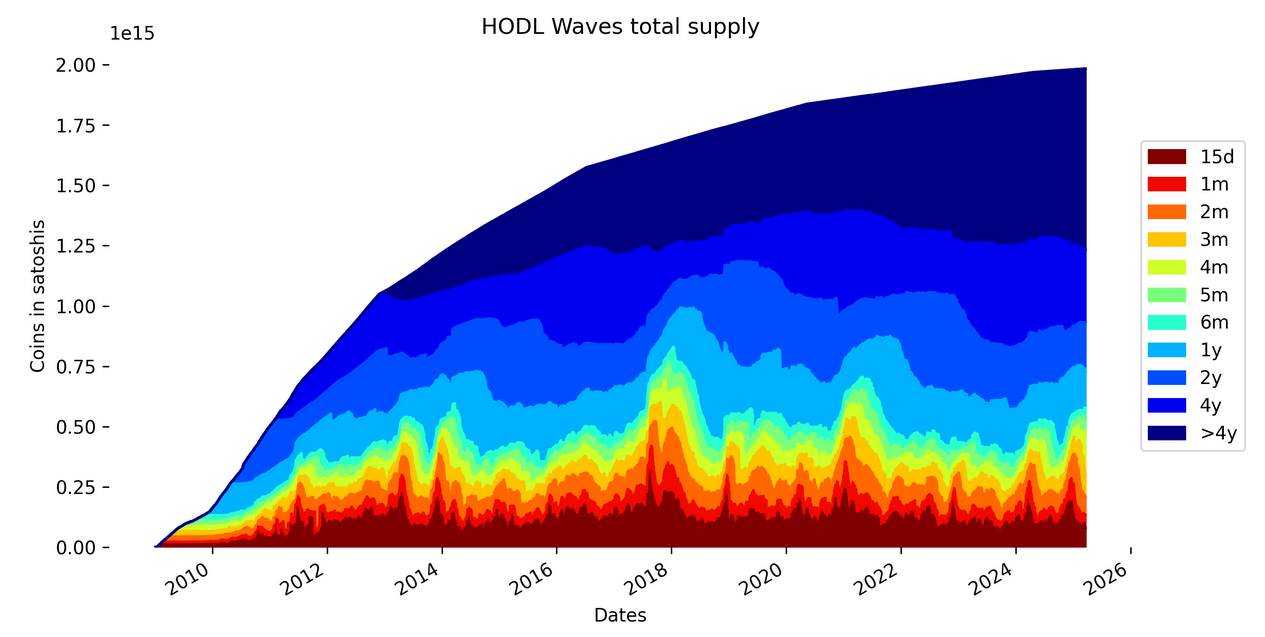
\includegraphics[width=\textwidth]{utxo-age}
\end{frame}

\begin{frame}
  \frametitle{Forks 1/2}
  \begin{itemize}
  \item \textbf{Soft fork} is a change to the Bitcoin protocol that
    \textbf{restricts} the set of rules applied to blocks and transactions:
    \begin{itemize}
    \item \textbf{some} of the blocks or transactions considered \textbf{valid} by the
      \textbf{old (non-upgraded) nodes} are considered \textbf{invalid} by the
      \textbf{new (upgraded) nodes},
    \end{itemize}
  \item Soft fork does not drop any nodes from consensus, but requires majority
    of the nodes to upgrade for the new rule to be enforced.
  \item Old nodes can still ``play by the old rules''.
  \end{itemize}
\end{frame}

\begin{frame}
  \frametitle{Forks 2/2}
  \begin{itemize}
  \item \textbf{Hard fork} is a change to the Bitcoin protocol that
    \textbf{relaxes} the set of rules applied to blocks and transactions:
    \begin{itemize}
    \item \textbf{some} of the blocks or transactions considered \textbf{valid}
      by the \textbf{new (upgraded) nodes} are considered \textbf{invalid} by
      the \textbf{old (non-upgraded) nodes},
    \end{itemize}
  \item Hard fork effectively drops old nodes from consensus, so it requires all
    nodes to upgrade to avoid the network split.
  \item Nodes that ``play by the old rules'' are split into a separate network.
  \end{itemize}
\end{frame}

\begin{frame}
  \frametitle{Network Hashrate}
  \begin{itemize}
  \item For \textbf{hash-based Proof-of-Work systems}, the computing power can
    be conveniently measured by \textbf{hashrate} - \textbf{hashes computed per
      second} (H/s).
  \item Current total \textbf{hashrate} of the Bitcoin network is approximately
    145 Eh/s ($145 \times 10^{18} = $ 145,000,000,000,000,000 H/s).
  \item As block rewards attract more miners, the total computing power of
    Bitcoin network increases.
  \end{itemize}
  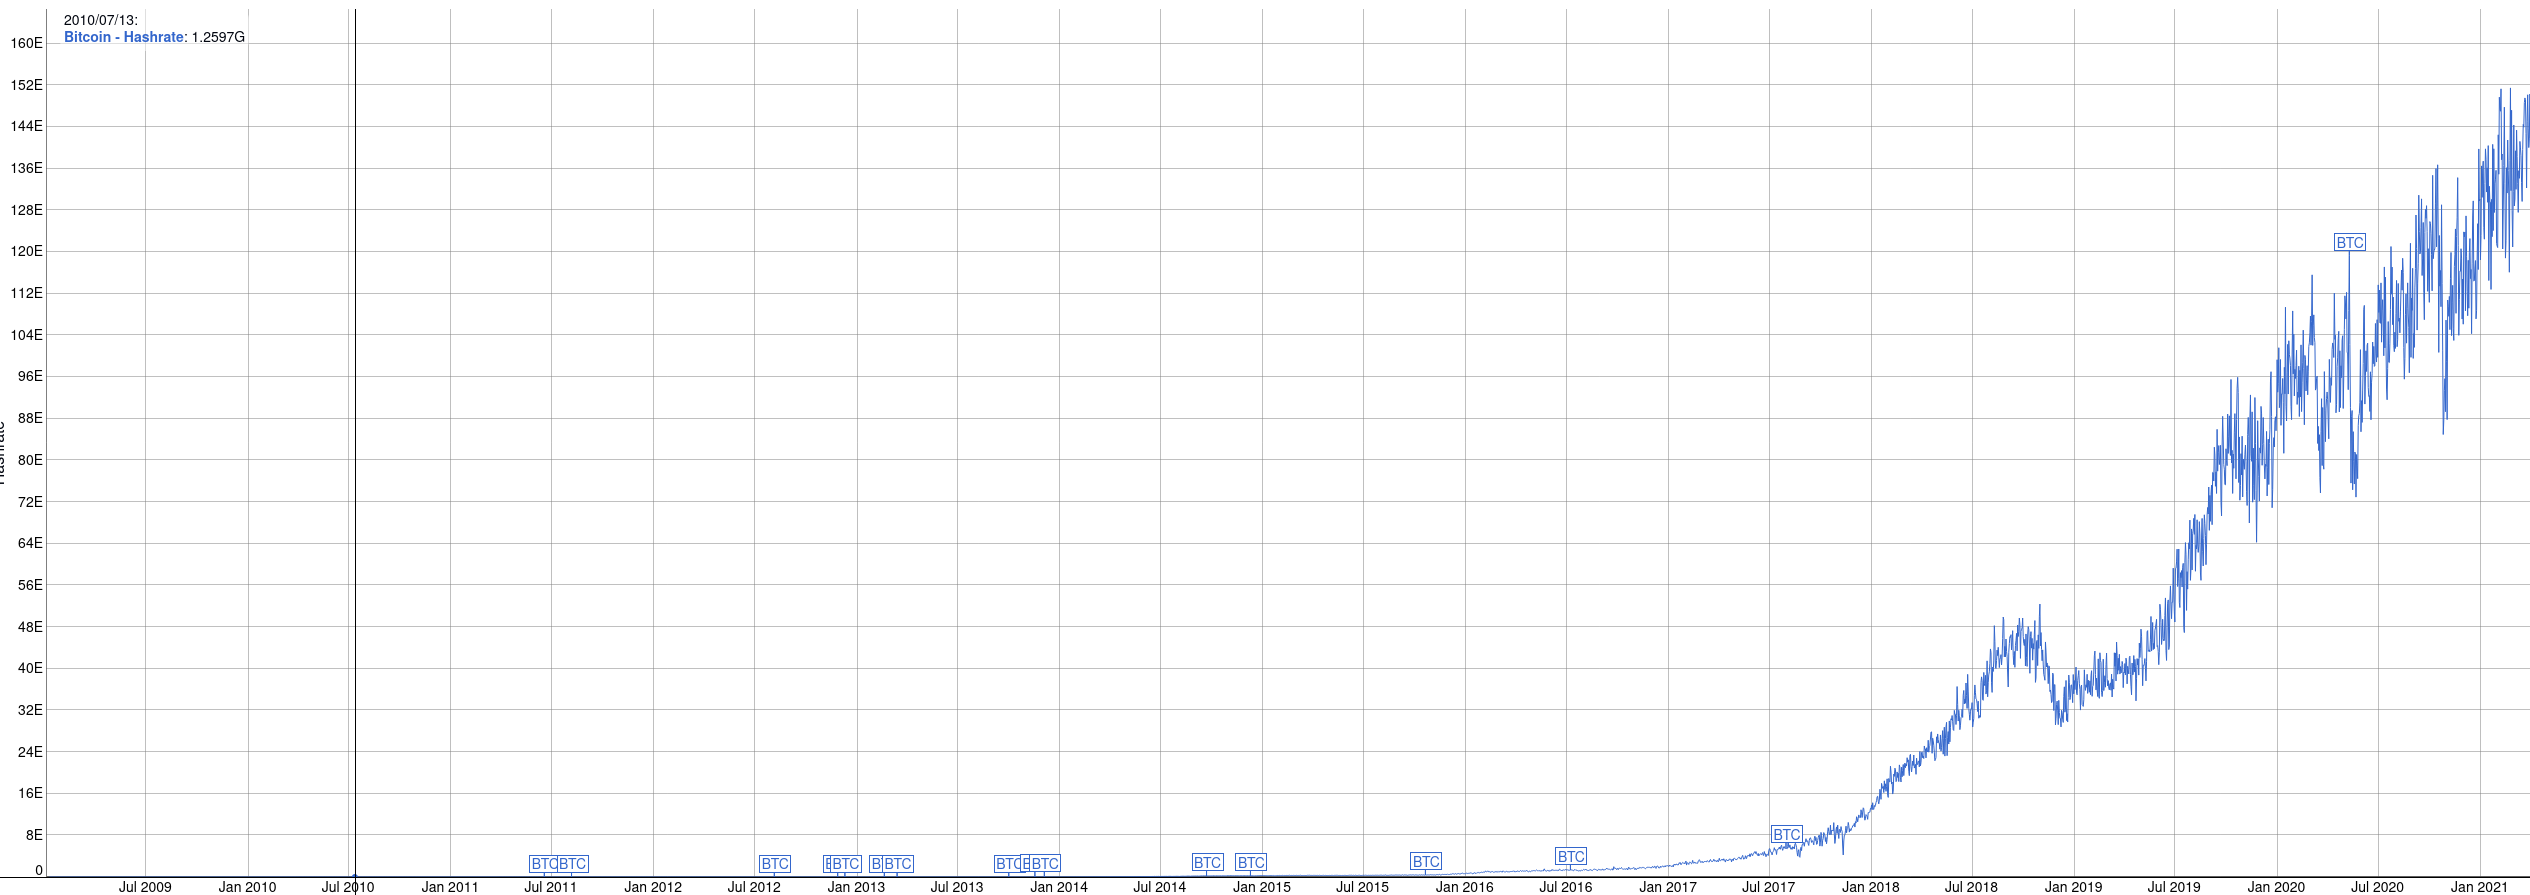
\includegraphics[width=\textwidth]{hashrate}
\end{frame}

\begin{frame}
  \frametitle{Difficulty Adjustment}
  \begin{itemize}
  \item In order to accomodate to the increasing computing power of the network,
    Bitcoin Protocol includes the \textbf{difficulty adjustment process}.
  \item Every 2,016 blocks (approximately 2 weeks), the difficulty of the PoW
    task is recalculated based on the last 2,016 blocks:
    \begin{itemize}
    \item if the averate time between last 2,016 blocks is \textit{more than 600
        seconds}, the \textit{difficulty is decreased} (the \textit{PoW target
        is increased}), otherwise the \textit{difficulty is increased} (the
      \textit{PoW target is decreased}).
    \end{itemize}
  \item The PoW difficulty is represented as the \textbf{PoW target} 256-bit
    number, which is in turn encoded as \textbf{bits} value and included in the
    block header, so the PoW solution can be verified independently.
  \end{itemize}
\end{frame}

\begin{frame}
  \frametitle{The End}
  \begin{center}
    Thank you!
  \end{center}
\end{frame}

\end{document}

%%% Local Variables:
%%% mode: latex
%%% TeX-master: t
%%% End:
